\iffalse
TODO:

- Magneten kaufen: http://www.amazon.de/Singende-Magnetsteine-Rattle-Snake-2er/dp/B00511MMY0/ref=sr_1_2?ie=UTF8&qid=1426673724&sr=8-2&keywords=zwitscher+magnete

- Datum

- Chirp center

- Simulation alt tab

alternative themes:
JuanLesPins
AnnArbor
Ilmenau

Ablauf:
1. Experiment + Erklärung + Simulation
2. Analyse erklären
	a. Chirp, Peak, PeakPeak
	b. Trennung von Frequenzen
		1. Chirp Frequenz (wann die Peaks kommen)
		2. Peak Frequenz (die Frequenz eines einzelnen Peaks)
3. Analyse
	a. Chirp Analyse
		1. Periodendauer ((Zeitabstände) (1/f)) --> e Funktion, Faktor wegen damped oszilation
		2. Amplitude über Zeit siehe oben, gleicher Faktor (Ungenauigkeiten)
		3. Gleichsetzung (Seite 10)
			a. Ansätze von den einzelnen Faktoren
			b. Ergebnisse
		4. Verallgemeinerung
			a. why
			b. Energie Ansatz
			c. Graph
	b. Peak Analyse
		1. Frequenz eines Peaks (siehe Nacharbeitung)
\fi


\documentclass[12pt]{beamer}
\usetheme{JuanLesPins}
\usepackage[utf8]{inputenc}
\usepackage[german]{babel}
\usepackage{amsmath}
\usepackage{amsfonts}
\usepackage{amssymb}
\usepackage{graphicx}
\usepackage{media9}
\usepackage{moresize}
\usepackage{hyperref}
\usepackage{xfrac}
\author{Leonard Hackel und Niklas Schelten}
\title{5. PK - Ball Sound}
\subtitle{Wie entwickelt sich der Ton, der beim Zusammenstoß zweier Metallkugeln entsteht?}
\setbeamertemplate{navigation symbols}{}
\logo{
\includegraphics[scale=0.028]{Bilder/Logo.png}} 
\institute{Herder Oberschule Berlin} 
\date{\today}
\subject{Physik} 

\newcommand{\multiplelines}[2][c]{\begin{tabular}[#1]{@{}l@{}}#2\end{tabular}}

%Frame numbers
\setbeamertemplate{footline}
{%
\begin{beamercolorbox}[wd=0.5\textwidth,ht=3ex,dp=1.5ex,leftskip=.5em,rightskip=.5em]{author in head/foot}%
\usebeamerfont{author in head/foot}%
\insertframenumber\ von \inserttotalframenumber\hfill\insertshortauthor%
\end{beamercolorbox}%
\vspace*{-4.5ex}\hspace*{0.5\textwidth}%
\begin{beamercolorbox}[wd=0.5\textwidth,ht=3ex,dp=1.5ex,left,leftskip=.5em]{title in head/foot}%
\usebeamerfont{title in head/foot}%
\insertshorttitle%
\end{beamercolorbox}%
}
%-------------------------------------------------------------------------------------------------
\begin{document}

\begin{frame}
\titlepage
\end{frame}

\begin{frame}
\tableofcontents
\end{frame}

%-------------------------------------------------------------------------------------------------
\section{Das Experiment}
\subsection{Vorführung}
\begin{frame}{Experiment}

\end{frame}

\subsection{Zusammensetzung des Tons}
\begin{frame}{\only<1-2>{Chirp}\only<3-4>{Peak}\only<5>{PeakPeak}}
\center{
\only<1>{\includemedia[addresource=Daten/Chirp.mp3, flashvars={source=Daten/Chirp.mp3&autoPlay=true}]
	{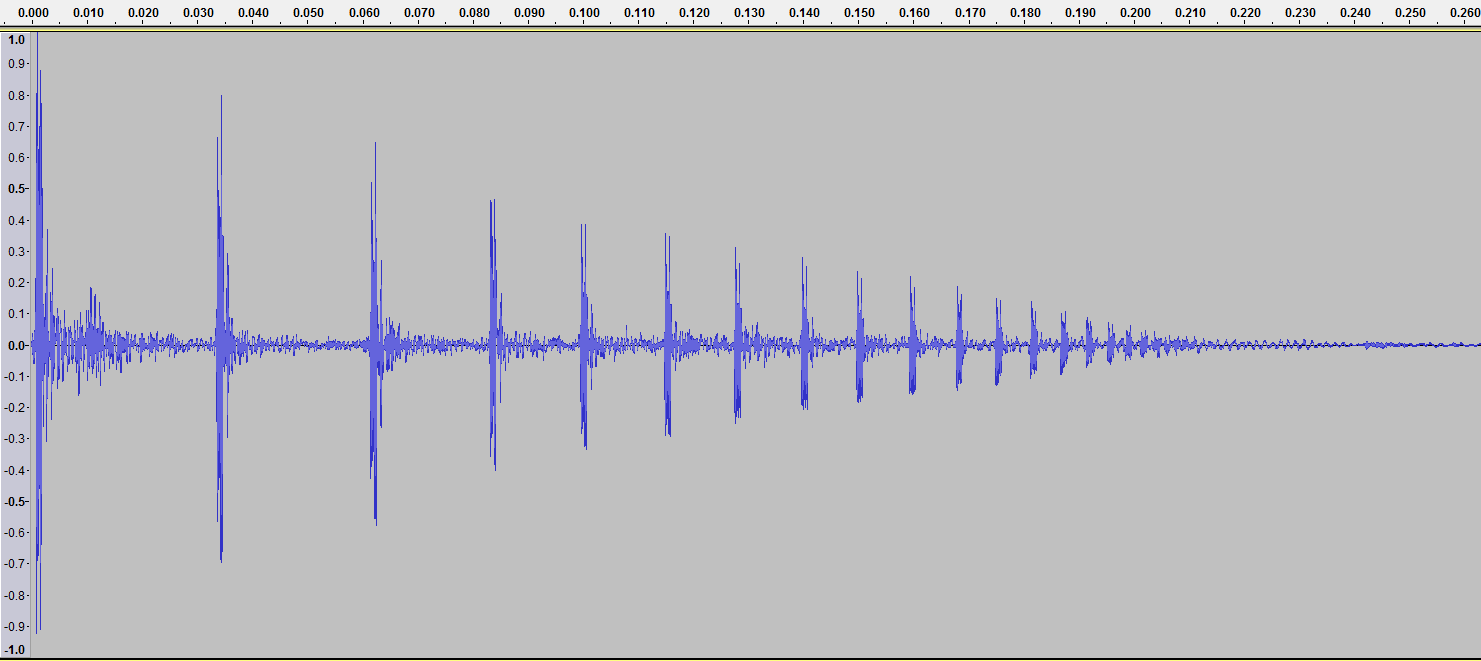
\includegraphics[scale=0.2]{Bilder/Chirp1.png}}{APlayer.swf}}
\only<2>{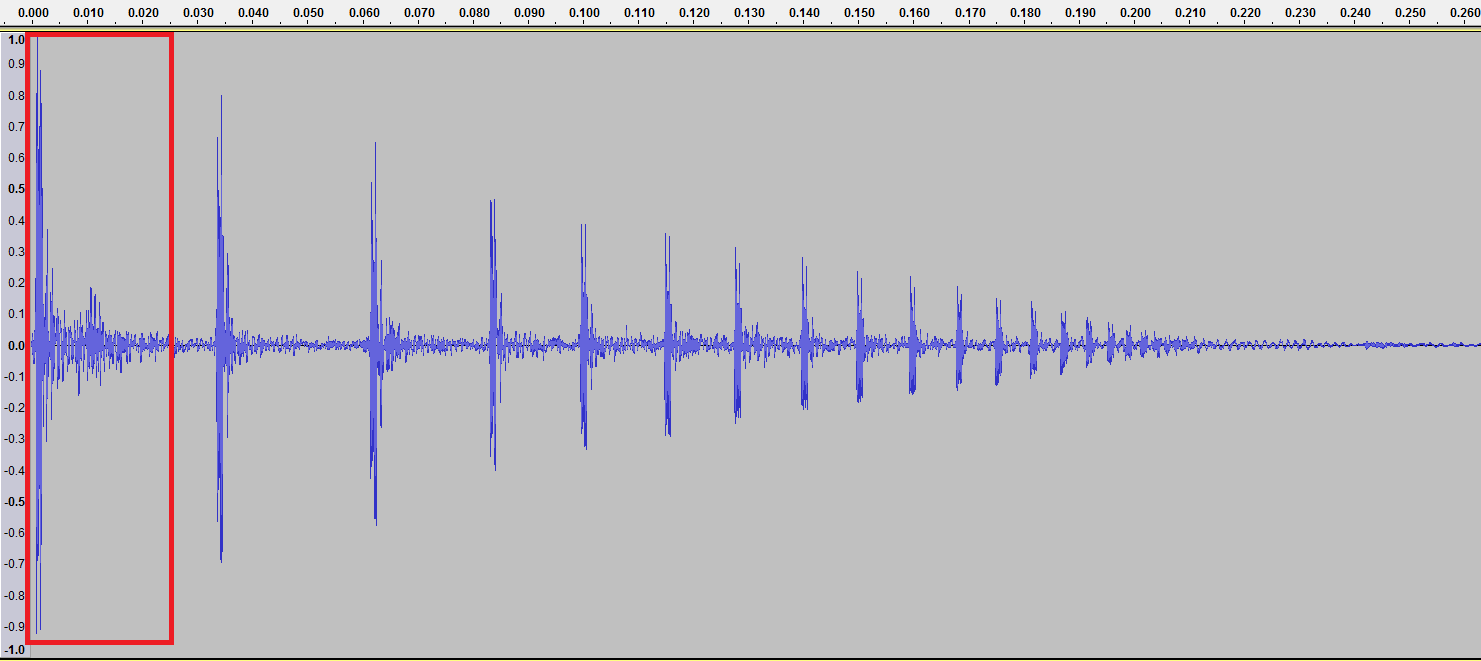
\includegraphics[scale=0.2]{Bilder/Chirp2.png}}
\only<3>{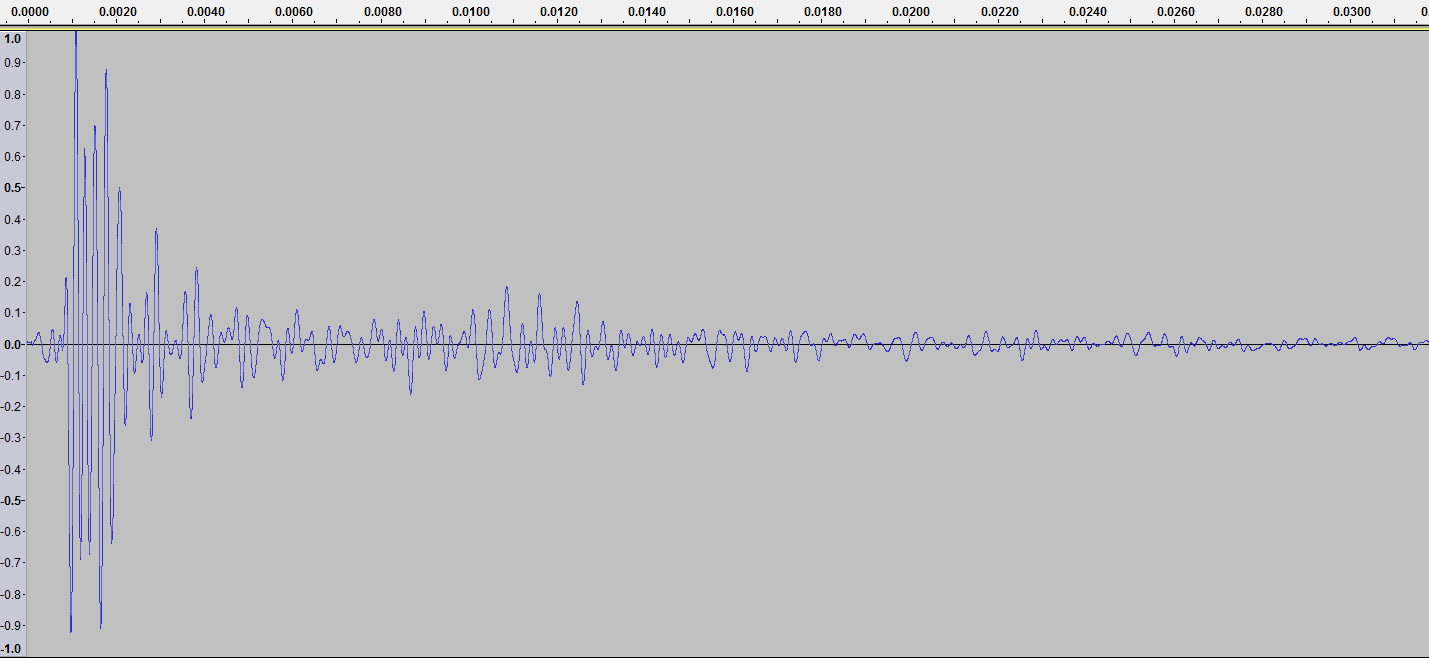
\includegraphics[scale=0.2]{Bilder/Peak1.png}}
\only<4>{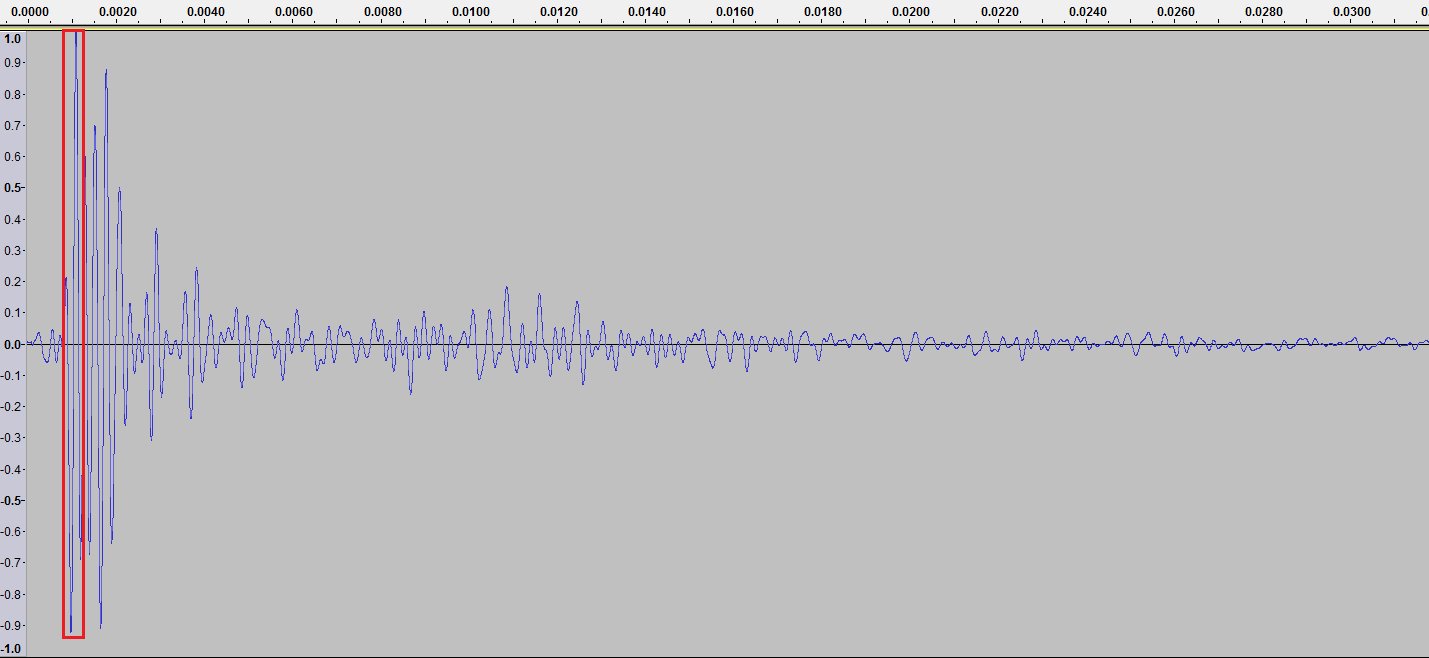
\includegraphics[scale=0.2]{Bilder/Peak2.png}}
\only<5>{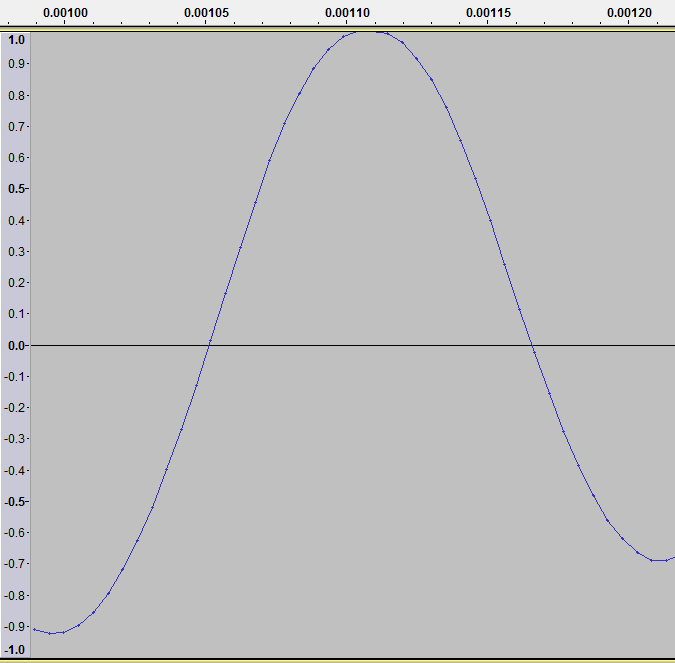
\includegraphics[scale=0.2]{Bilder/PeakPeak.png}}
}
\end{frame}

\begin{frame}{Frequenzen}
\begin{itemize}
\item<1-> Chirp Frequenz
	\begin{itemize}
	\item<2->[$\rightarrow$] Anzahl der Peaks pro Sekunde
	\end{itemize}
\item<3-> Peak Frequenz
	\begin{itemize}
	\item<4->[$\rightarrow$] Anzahl der PeakPeaks pro Sekunde
	\end{itemize}
\end{itemize}
\end{frame}

\subsection{Simulation}
\begin{frame}{Simulation}
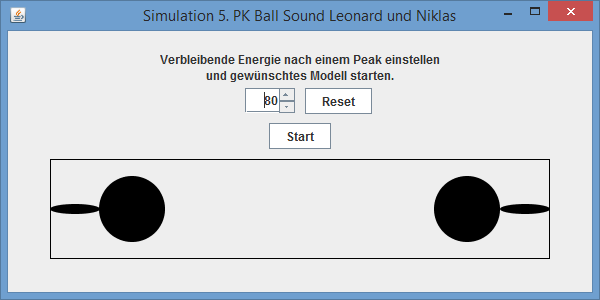
\includegraphics[scale=0.5]{Bilder/Simulation.png}
\end{frame}
%-------------------------------------------------------------------------------------------------
\section{Physikalische Analyse}
\subsection{Chirp}
\subsubsection{Physikalische Beschreibung des Tons}

\begin{frame}{Periodendauer über Peaks}
\begin{columns}
\begin{column}{.55\textwidth}
	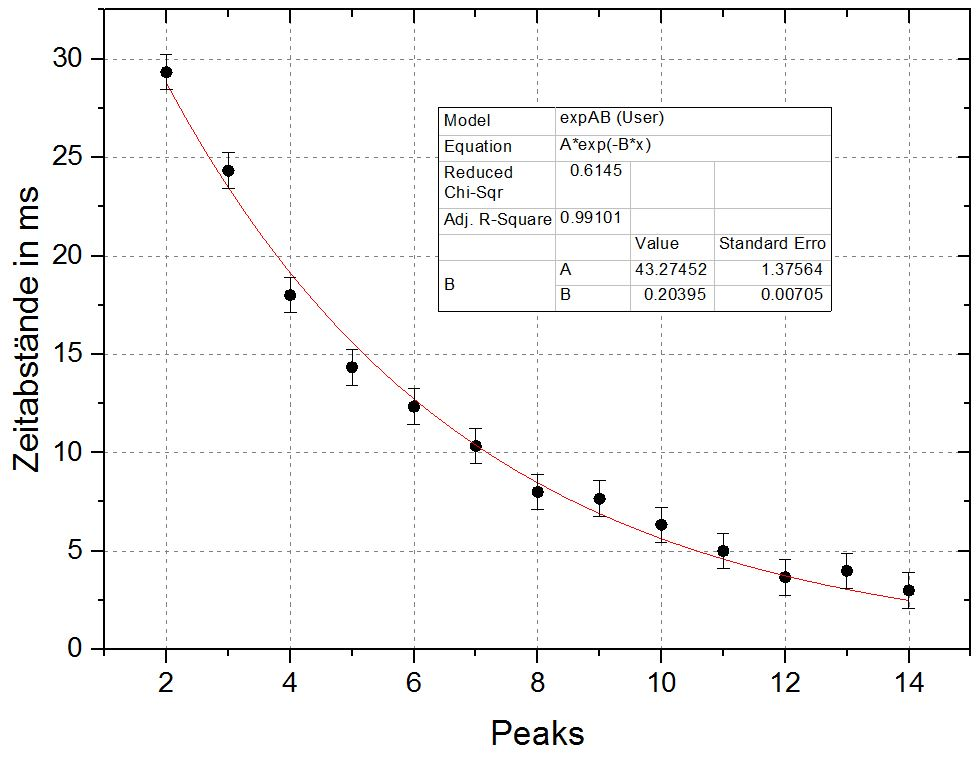
\includegraphics[scale=0.265]{Bilder/Periodendauer.jpg}
\end{column}
\begin{column}{.45\textwidth}
	\begin{itemize}
	\item<1-> $\delta_{fit}(x)=43,27\cdot 0,82^x$
	\item<2-> $\delta_n=\delta_1\cdot b^{n-1}$
		\begin{itemize}
		\item $0\leq b<1$
		\item $n$: Anzahl der Peaks
		\item $\delta$: Periode
		\end{itemize}
	\item[ ] \ %just for moving the lines up ^_^
	\end{itemize}
\end{column}
\end{columns}
\end{frame}

\begin{frame}{Amplitude über Peaks}
\begin{columns}
\begin{column}{.55\textwidth}
	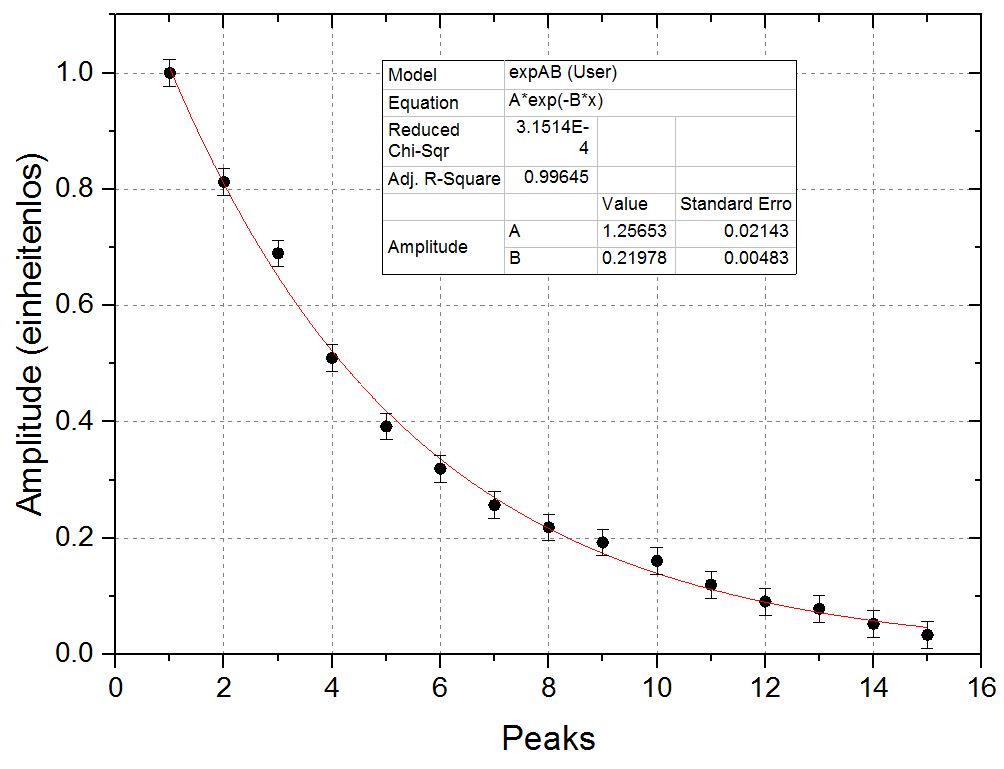
\includegraphics[scale=0.26]{Bilder/Amplitude.jpg}
\end{column}
\begin{column}{.45\textwidth}
	\begin{itemize}
	\item<1-> $y_{fit}(x)=1,26\cdot 0,80^x$
	\item<2-> $y_n=a\cdot y_{n-1}$
		\begin{itemize}
		\item $0\leq a<1$
		\item $n$: Anzahl der Peaks
		\item $y$: Amplitude
		\end{itemize}
	\item<3->[$\Rightarrow$] $y_n=y_0\cdot a^n$
	\end{itemize}
\end{column}
\end{columns}
	
\end{frame}

\begin{frame}{Amplitude in Abhängigkeit von der Periode}
\begin{itemize}
\item Beide Gleichungen nach $n$ umformen, gleichsetzen \only<2>{und nach $y_n$ umformen:}
	\begin{itemize}
	\item[$\rightarrow$]
		\only<1>{$\frac{\log\frac{y_n}{y_0}}{\log a}=\frac{\log\left(1-\frac{t_n}{t_{ges}}\right)}{\log b}$}
		\only<2>{$y_n=y_0\cdot\left(1-\frac{t_n}{t_{ges}}\right)^{\frac{\log a}{\log b}}$}
	\end{itemize}
\end{itemize}
\end{frame}

\subsubsection{Verallgemeinerung}
\begin{frame}{Verallgemeinerung - Was haben wir davon?}
\begin{columns}
\begin{column}{0.6\textwidth}
	\begin{itemize}
	\item<1-> unterschiedliche rücktreibende Kräfte \only<5->{$\rightarrow$ Potenz des Weges}
		\begin{itemize}
		\item<2->[-] Gravitation \only<6->{$\rightarrow$ nahezu $s^0$}
		\item<3->[-] Magnetkraft \only<7->{$\rightarrow$ $s^{-2}$}
		\item<4->[-] Federkaft \only<8->{$\rightarrow$ $s^1$}
		\end{itemize}
	\end{itemize}
\end{column}
\begin{column}{0.4\textwidth}
	\only<3>{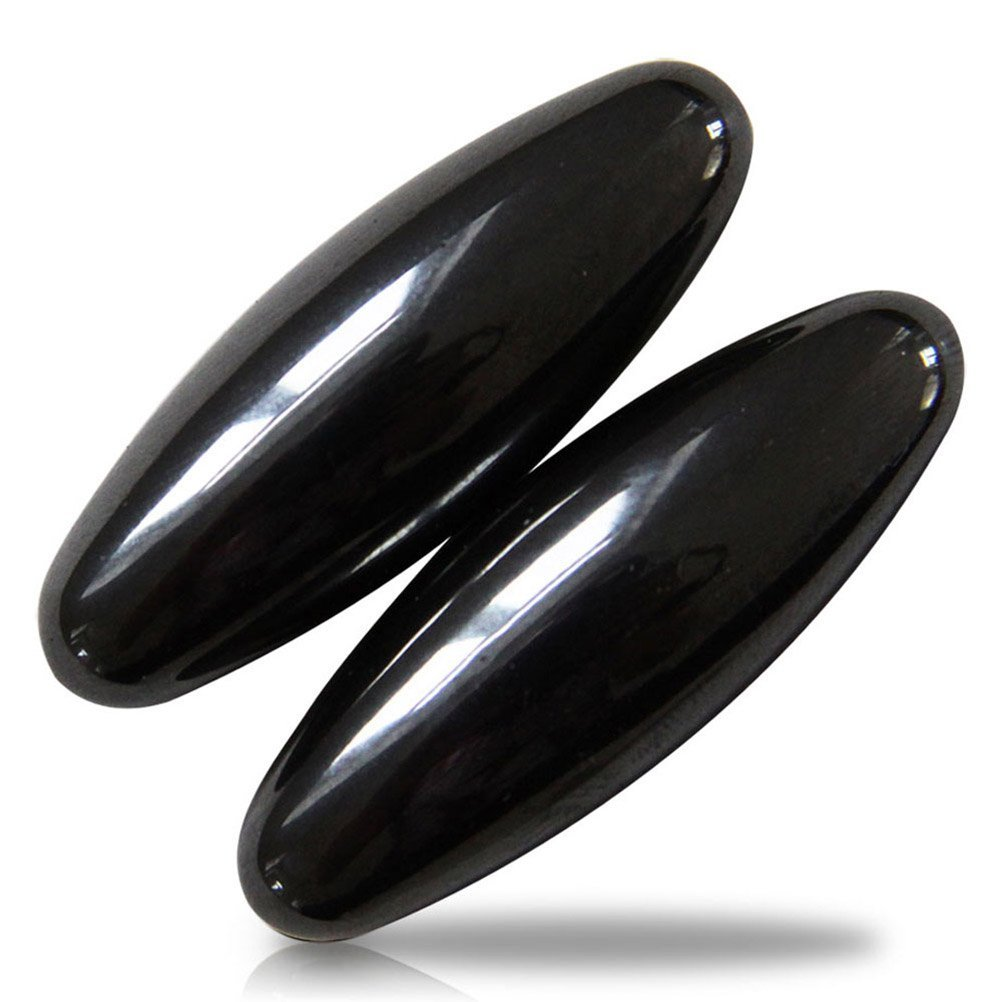
\includegraphics[scale=0.1]{Bilder/Magnete.jpg}}
	\only<4>{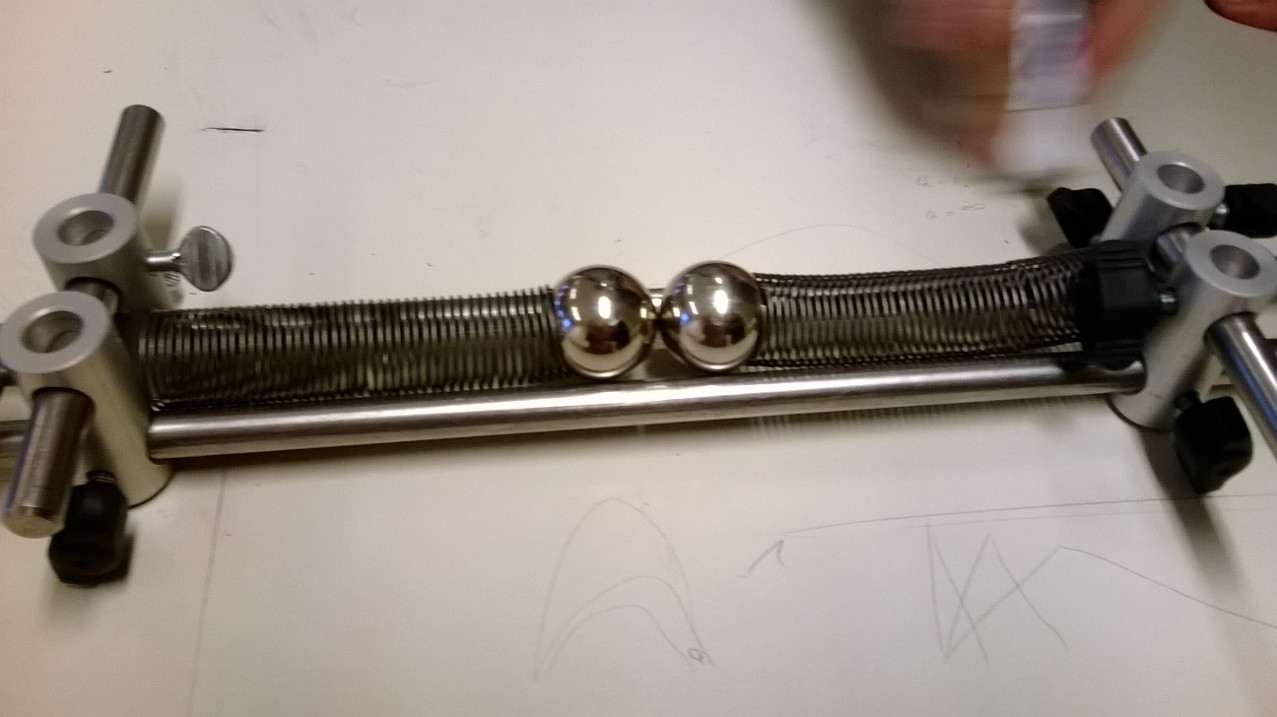
\includegraphics[scale=0.1]{Bilder/Feder.jpg}}
\end{column}
\end{columns}
\end{frame}

\begin{frame}{Verallgemeinerung - Differentialgleichung}
\begin{itemize}
\item<1-> folgende Differentialgleichung als Ergebnis:
	\begin{itemize}
	\item<1-> $m\cdot \ddot{s}+c\cdot s^a=0$
	\end{itemize}
\end{itemize}
\end{frame}

%jeden graphen einzeln anzeigen
\begin{frame}{Verallgemeinerung - Ergebnis}
\only<1>{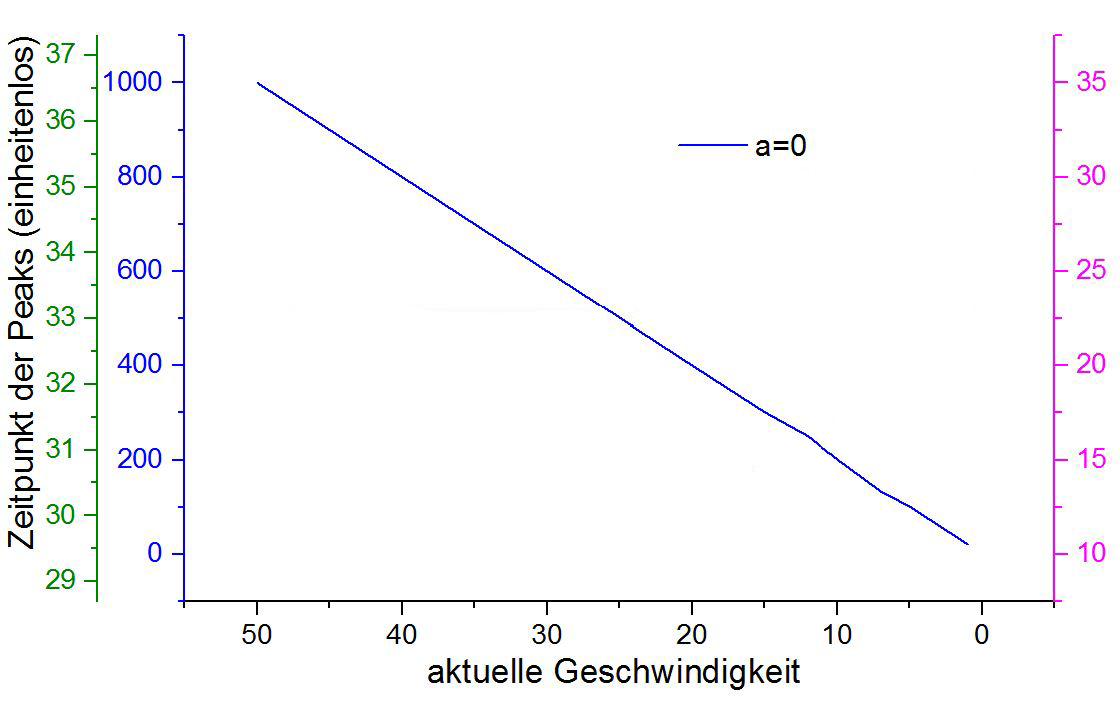
\includegraphics[scale=0.2]{Bilder/Diff'Gleichung(0).jpg}}
\only<2>{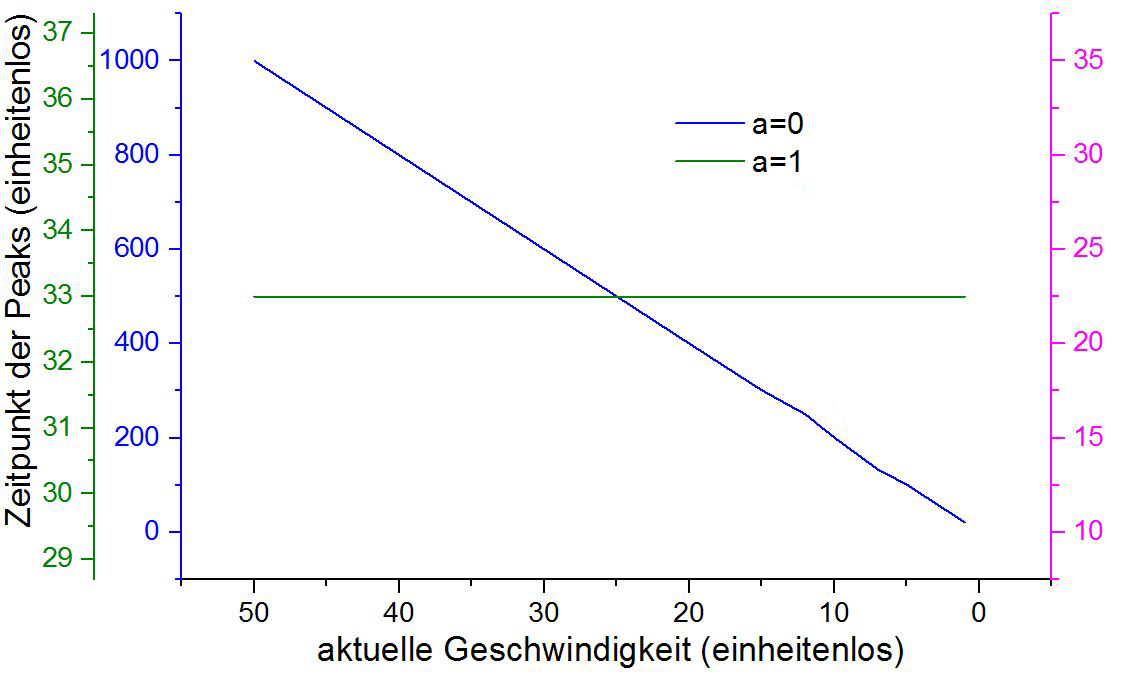
\includegraphics[scale=0.2]{Bilder/Diff'Gleichung(01).jpg}}
\only<3>{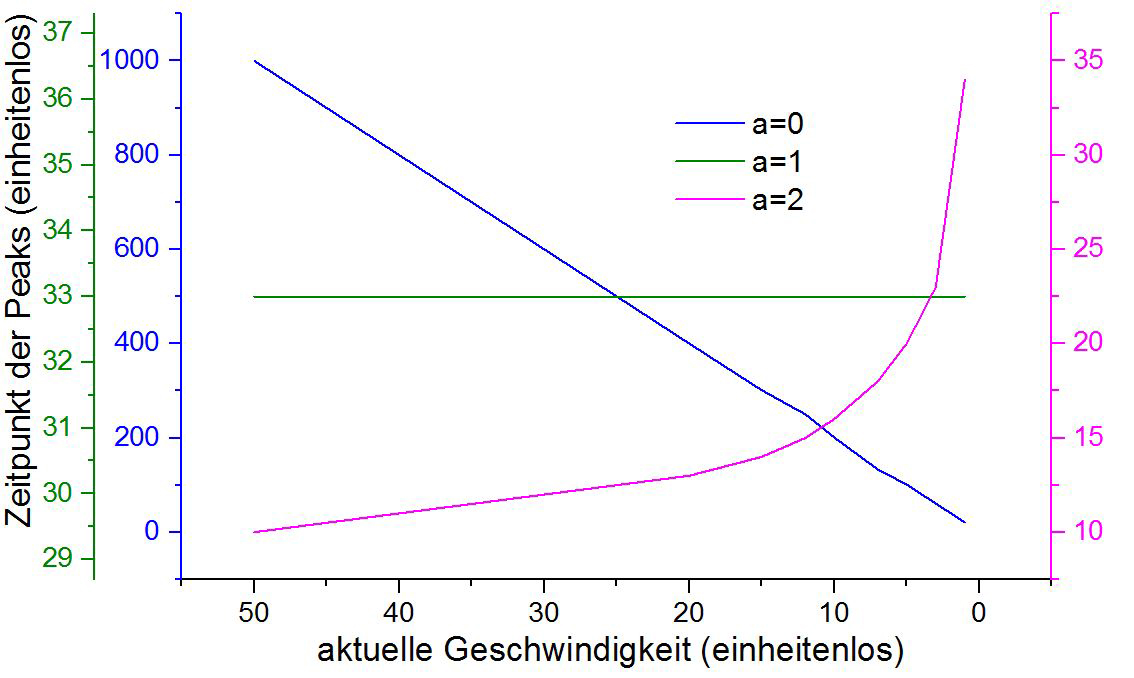
\includegraphics[scale=0.2]{Bilder/Diff'Gleichung(012).jpg}}
\end{frame}

\subsection{Peak}
\subsubsection{Frequenz}
\begin{frame}{Frequenz}
\begin{itemize}
\item<1-> Peak-Frequenz für jeden Peak gleich
\item<2-> zwei Ursprünge:
	\begin{itemize}
	\item<2-> Eigenfrequenz der Kugeln
	\item<3-> Frequenz zwischen den Kugeln
	\end{itemize}
\end{itemize}
\end{frame}

\begin{frame}{Eigenfrequenz}
\begin{itemize}
\item<1-> stehende Welle in den Kugeln
	\begin{itemize}
	\item<2->[$\rightarrow$] $f=\frac{c}{2n\cdot\lambda}=\frac{5170\sfrac{m}{s}}{8\cdot 0,017m}\approx 38kHz$ mit $n\in \mathbb{N}$
	\item<3->[$\rightarrow$] nicht hörbar
	\end{itemize}
\end{itemize}
\end{frame}

\begin{frame}{"`Auftreff Frequenz"'}
\begin{itemize}
\item<1-> Arbeit von K. Mehraby, H Khadem-hosseini Beheshti und M. Poursina\footnotemark
	\begin{itemize}
	\item<2->[$\rightarrow$] $f=\frac{76,1}{r}Hz=\frac{76,1}{0,017}Hz\approx 4476Hz$
	\end{itemize}
\end{itemize}
\footnotetext[1]{\href{http://www.researchgate.net/profile/Mehrdad_Poursina/publication/225820012_Impact_noise_radiated_by_collision_of_two_spheres_Comparison_between_numerical_simulations_experiments_and_analytical_results/links/00463527e9e985bfd2000000}{\tiny Impact noise radiated by collision of two spheres: Comparison between numerical\\
\vspace{-3pt}\hspace{18pt}simulations, experiments and analytical results}}
\end{frame}

\begin{frame}{Frequenzanalyse}
\begin{columns}
\begin{column}{.6\textwidth}
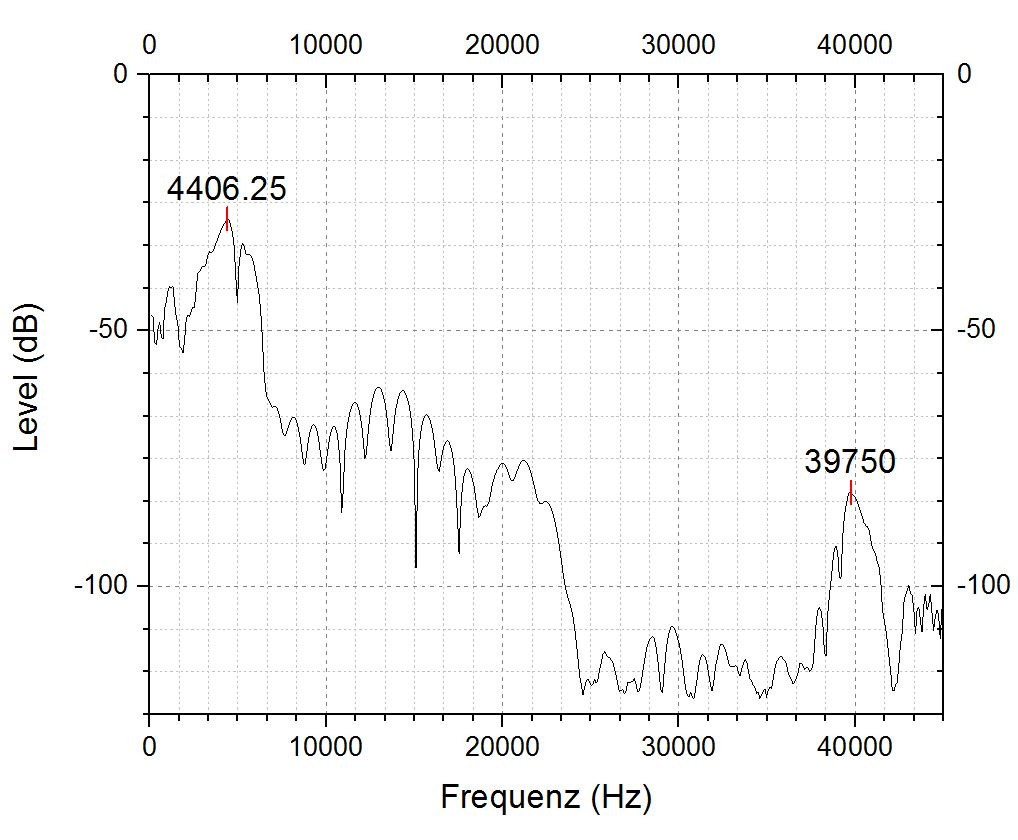
\includegraphics[scale=0.28]{Bilder/Frequenzen.jpg}
\end{column}
\begin{column}{.4\textwidth}
\begin{itemize}
\item<2-> hörbare Frequenz $4406Hz$ "`Auftreff Frequenz"'
\item<3-> nicht hörbare Frequenz $39kHz$ Eigenfrequenz
\item[ ] \ 
\end{itemize}
\end{column}
\end{columns}
\end{frame}

\begin{frame}
\center
{\HUGE Vielen Dank für Ihre Aufmerksamkeit}
\end{frame}
\end{document}